

\section{Introduction}
\label{sec:introduction}

The quantitative understanding of the physical world is an essential goal of geoscience research. We use mathematical abstractions to represent the behavior of systems under static and dynamic conditions; and properties such as density and elastic moduli to characterize the capacity of materials to absorbe or transmit forces in stationary and transient processes. In seismology and geophysics, our understanding of physical phenomena associated to earthquakes, their genesis, and effects, depends in a good measure on our knowledge and accurate representation of the geometry and material properties of the Earth's structure, as well as on our capacity to represent the mechanical characteristics of the rupture process that takes place when a seismic fault breaks and the subsequent seismic wave propagation problem. We use stress conditions and dynamic rupture models to describe faulting processes; and seismic velocity and attenuation models, along with wave propagation principles to determine the characteristics of the ground motion.

Initial stress models and seismic velocity models are therefore at the most basic input-level in earthquake ground motion simulation. We are interested in how seismic velocity models are built and made available to geoscientists, and in particular, on how these models can help advance physics-based earthquake science. We utilize modeling approaches based on deterministic numerical techniques---such as the finite element, finite difference, or spectral element methods---to simulate the ground motion in ways that incorporate the physics of earthquake processes explicitly. That is, methods that explicitly solve the associated wave propagation problem. The use of physics-based earthquake simulation has increased considerably over the last two decades thanks to the growth---in capacity and availability---of high-performance computing (HPC) facilities and applications \citep[e.g.,][]{Aagaard_2008_BSSA2, Olsen_2009_GRL, Bielak_2010_GJI, Cui_2010_Proc}. These simulations have specific applications of great impact in seismology and earthquake engineering in aspects such as the assessment of regional seismic hazard \citep[e.g.,][]{Graves_2011_PAG}.

Recent simulations have highlighted the importance of velocity models in the accuracy of simulation results \citep[e.g.,][]{Taborda_2014_BSSA}. Numerous seismic velocity models have been built for specific regional or local structures and used in particular simulations over the years \citep[e.g.,][]{Frankel_1992_BSSA, Brocher_2008_BSSA, Graves_2008_BSSA}. The need for these models in simulation gave way to the conception of community velocity models (CVMs). CVMs are seismic velocity models that have been developed, maintained, advanced and used by a community of interested investigators. Some examples of CVMs for the regions of southern and northern California, Utah, and the central United States are those models developed by \citet{Kohler_2003_BSSA}, \citet{Suss_2003_JGR}, \citet{Brocher_2006_Proc}, \citet{Magistrale_2006_Tech}, \citet{RamirezGuzman_2012_BSSA}, and \citet{Plesch_2011_SCEC}. 

CVMs have been typically distributed in the form of datasets or collections of files, or in the form of computer programs that can dynamically operate on these datasets and files to provide information about the geometry and material properties of the crust in a particular region. However, these datasets and computer programs have not always been designed carefully from a computational perspective. In addition, recent advances in earthquake simulations, powered by the increasing capability of supercomputers, have increased significantly the computational demand placed on CVMs as input to these simulations. 

This paper presents the Unified Community Velocity Model (UCVM), a software framework designed to provide standardized and computationally efficient access to seismic velocity models, developed and maintained by the Southern California Earthquake Center (SCEC). UCVM is a collection of software tools and application programming interfaces (APIs) that facilitate the access to the material properties stored in CVMs. Although UCVM was conceived as a tool to aid physics-based earthquake ground-motion simulation and regional seismic hazard assessment, it can be and has been used in other geoscience and engineering applications. Here, we describe the development of UCVM and its various software components and features, including some for use in high-performance parallel computers, and present examples of recent applications of UCVM tools in geoscience and earthquake engineering research.




\begin{figure*}[ht!]
	\centering
	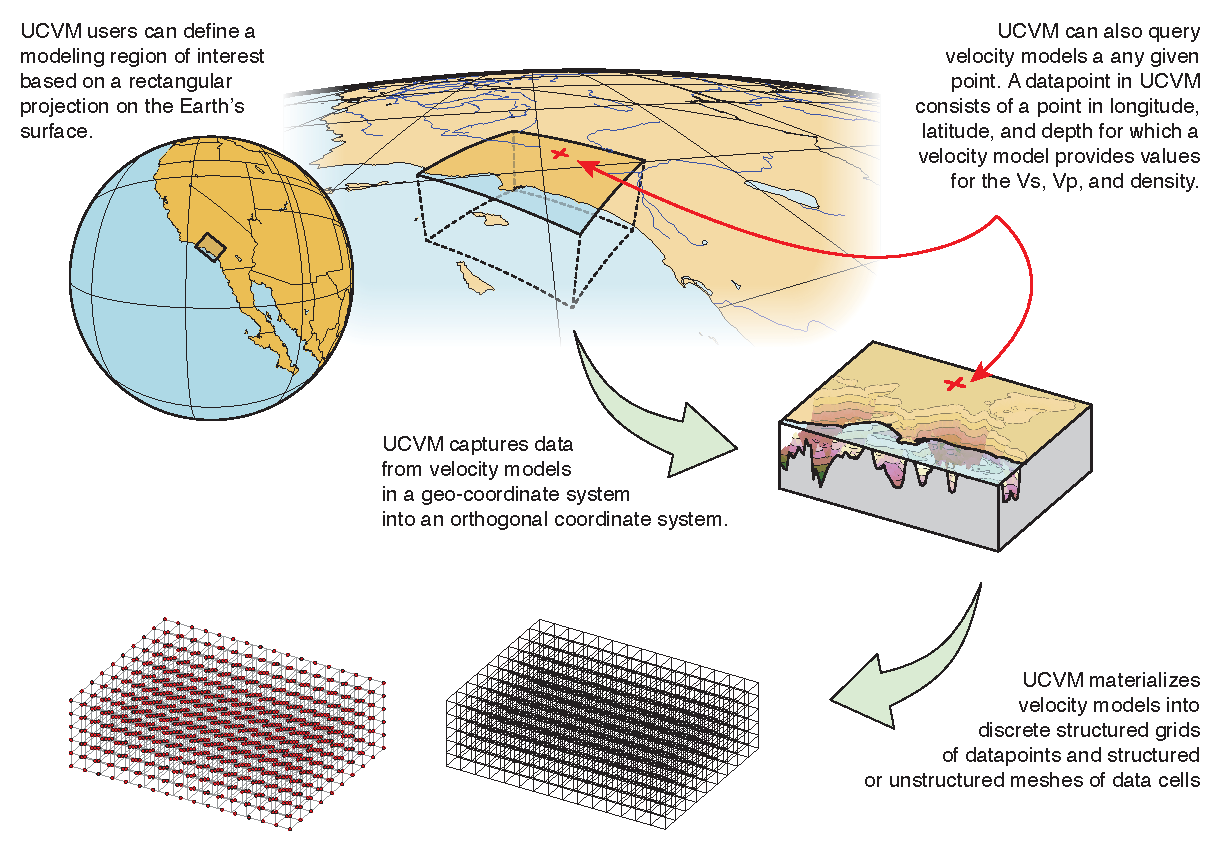
\includegraphics
		[width=0.9\textwidth]
		{figures/pdf/ucvm-model-extraction}
	\caption{High-level description of the UCVM framework functionality illustrating the selection of a region of interest for which a user can obtain datapoints using the UCVM utilities and create materialized models in the form of discrete three-dimensional grids or meshes.}
	\label{fig:framework}
\end{figure*}




\begin{figure*}[ht!]
	\centering
	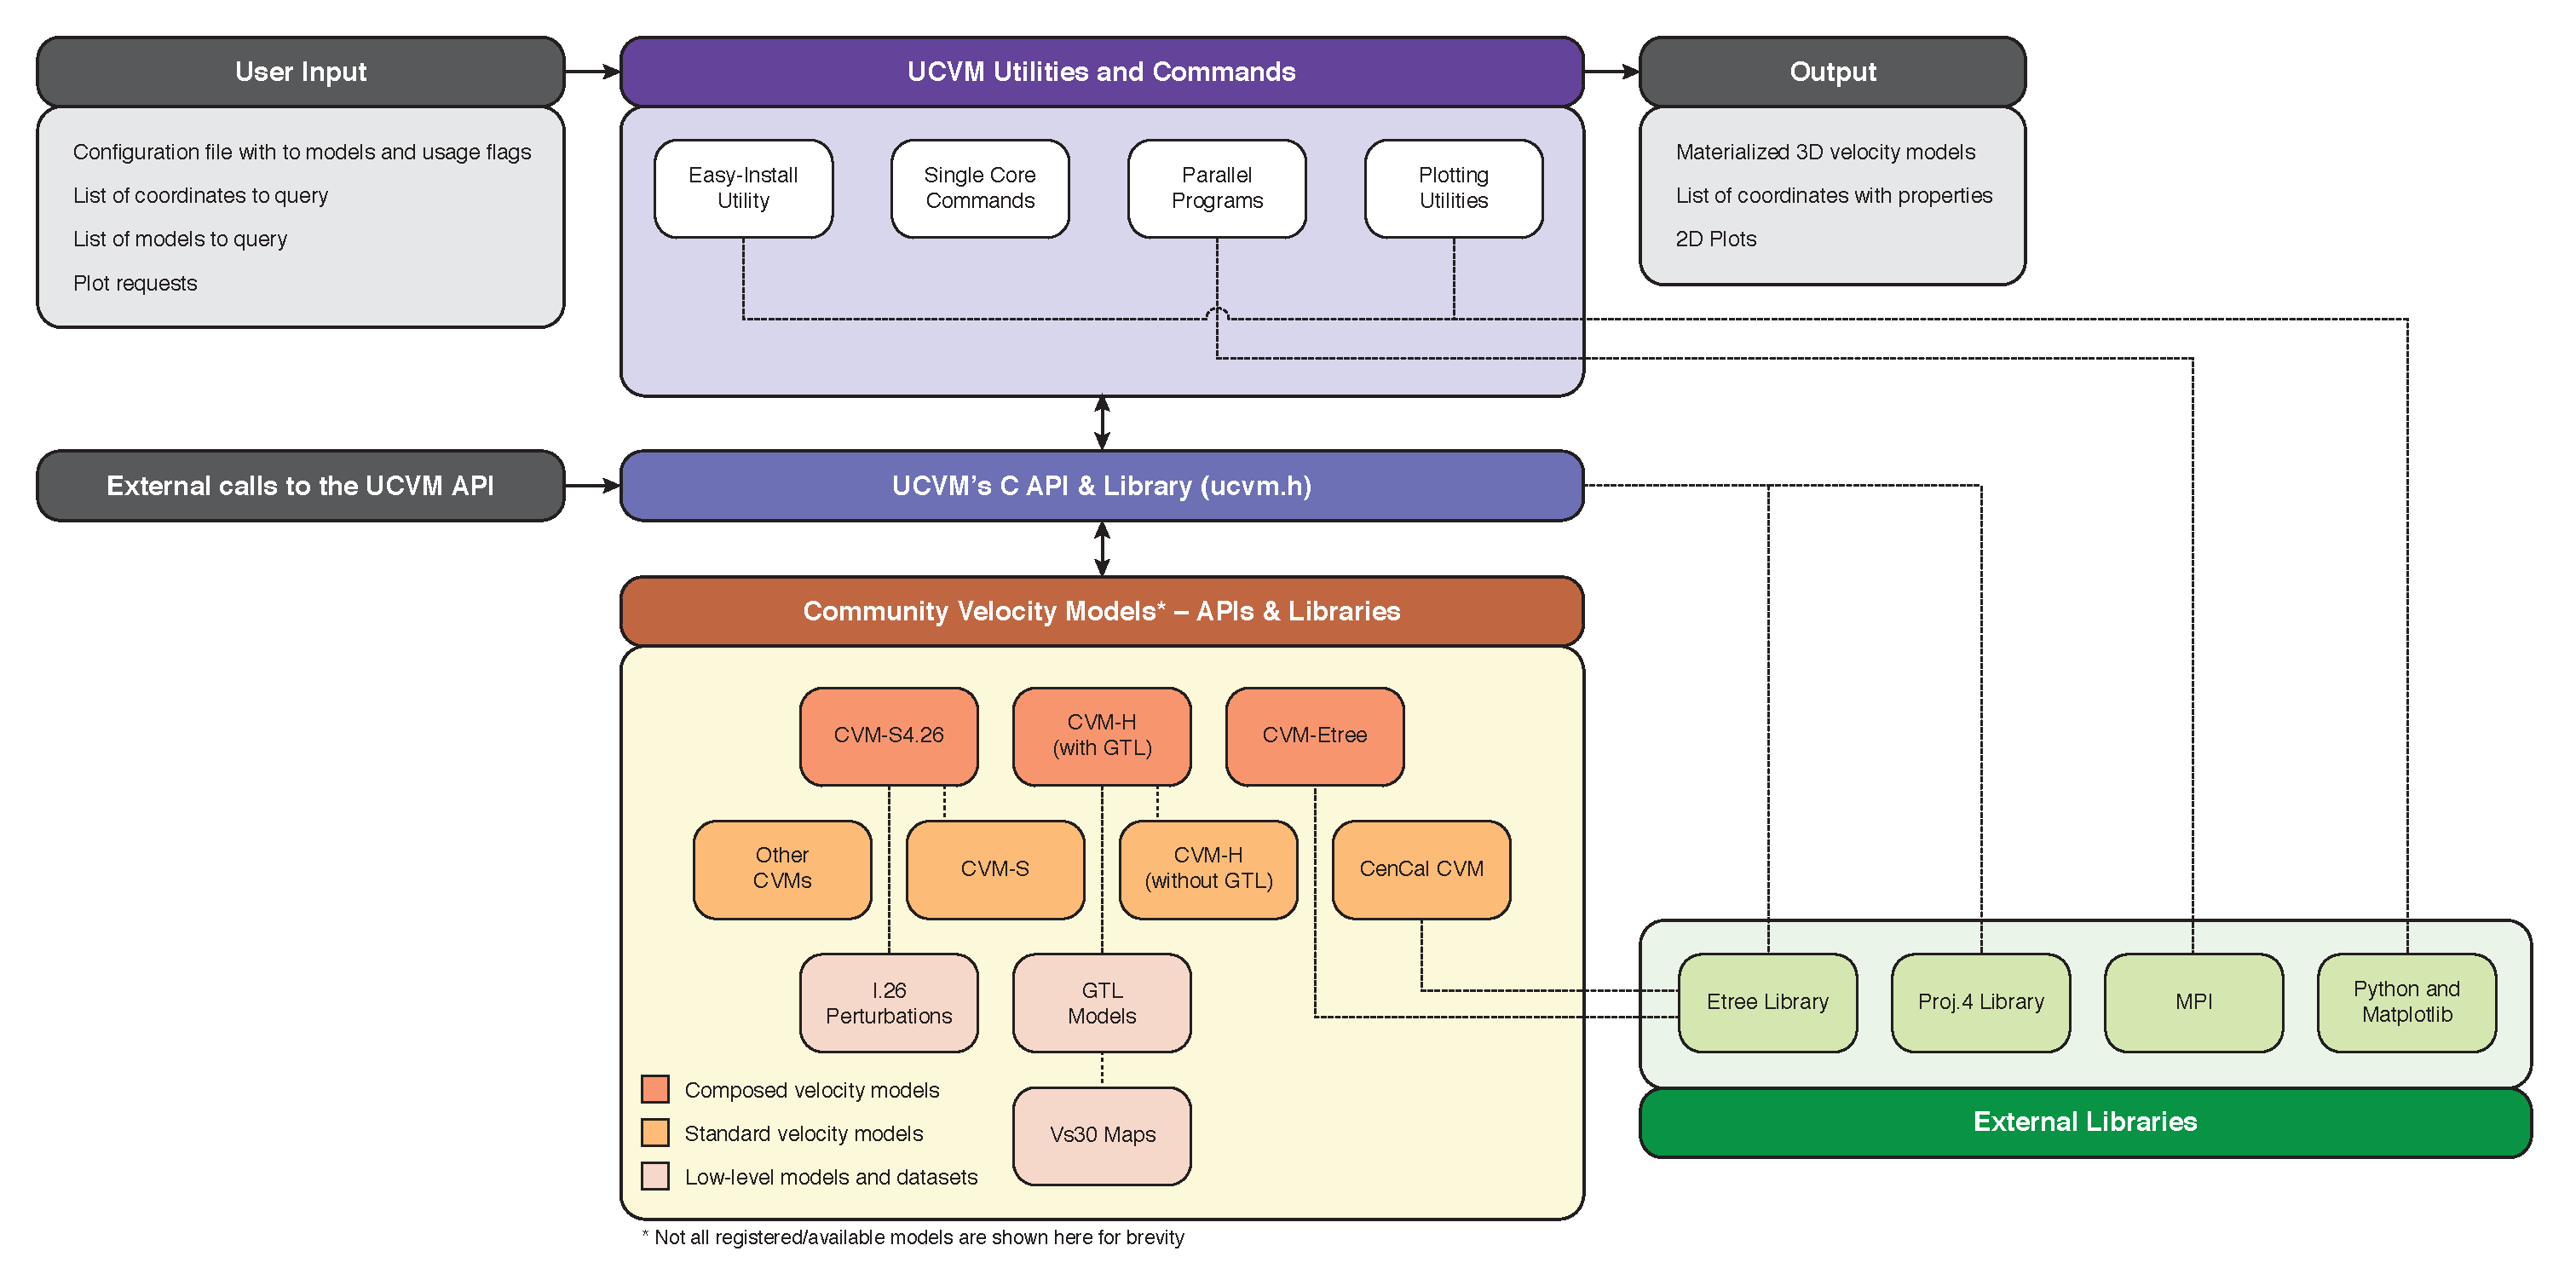
\includegraphics
		[width=\textwidth]
		{figures/pdf/ucvm-sw-architecture}
	\caption{The UCVM software architecture. Gray-colored frames indicate components at the level of user or client interaction. The upper purple-colored frame displays UCVM utilities and commands directly accessible to users, whereas the ligher purpled-colored box indicates the lower-level UCVM API and library upon which UCVM operations rest. Underlying this, are a selection of community models supported by UCVM; and to the right, in green, are the library dependencies of the UCVM framework. Here we distinguish models and datasets in four categories related to their origin or operational concept. In practice, however, UCVM treats each model or dataset independently and without any distinction.}
	\label{fig:sw.arch}
\end{figure*}



\begin{table*}[t]
\centering
\small
\caption{Electronic addresses to UCVM on-line documentation.}
\begin{tabular}[]{ll}
\\
Description                 & URL Address                                                         \\
\hline
General Documentation       & \url{http://scec.usc.edu/scecpedia/UCVM}                            \\
General User Guide          & \url{http://scec.usc.edu/scecpedia/UCVM_User_Guide}                 \\
Advanced User Guide 	    & \url{http://scec.usc.edu/scecpedia/UCVM_Advanced_User_Guide} 	  \\
Tutorial 	            & \url{http://scec.usc.edu/scecpedia/UCVM_Tutorial}            	  \\
Model Integration           & \url{http://scec.usc.edu/scecpedia/UCVM_Model_Integration_Guide}    \\
\hline
\end{tabular}
\label{tab:manuals}
\end{table*}


\section{The UCVM Software Framework}\label{sec:ucvm}

The primary functionality provided by UCVM is the ability to query a wide array of CVMs for material properties through a standardized query interface, and return material properties from the CVMs in standardized formats, independently of the particularities of each dataset or CVM. UCVM achieves this by registering datasets and velocity models into the framework. Registration of a velocity model or dataset consists of creating the appropriate API to facilitate the communication between the framework utilities and tools, and the velocity models and datasets. Once a velocity model or dataset has been registered with UCVM, a client can use the framework utilities to retrieve information from the models at any geographic point within the coverage region of the model(s). A client can be either a user (via the command-line) or a software application. The primary data type retrieved by a UCVM client for a single geographical point consists of a float triplet with the seismic velocities (\vp{} and \vs{}), and the material's density ($\rho$). At times we refer to this triple as the payload. The UCVM can then be used to produce standardized output in the form of three-dimensional (3D) volumetric datasets, two-dimensional (2D) vertical cross-sections and horizontal slices, and individual data points. This process is illustrated at a general level for the cases of 3D models in Figure \ref{fig:framework}. A client can also use other UCVM utilities for plotting and transforming models and datasets.

In order to facilitate access to the models, UCVM conceals each model's local coordinate system behind a generic querying interface. Data points are queried through this interface by geographic latitude and longitude, and a vertical $z$-coordinate. The framework allows defining the $z$-axis as either depth below the free surface (in meters, positive downward) or elevation relative to mean sea level (where zero is at sea level, positive upward and negative downward). The UCVM standardized interface allows multiple velocity models to be aggregated into a single composite model or meta-model. Composition is accomplished by tiling two or more velocity models in three dimensions according to a user-specified priority order. To support this flexible query mechanism consistently across all models, UCVM includes a high-resolution digital elevation model (DEM) and uses a cartographic projection library (Proj.4: \url{http://trac.osgeo.org/proj}). The DEM is synthesized from the USGS National Elevation Dataset \citep{Gesch_2002_PERS, Gesch_2007_Chap} and the ETOPO1 Global Relief Model \citep{Amante_2009_Manual}. The built-in DEM enables clients to retrieve the surface elevation at any query point in addition to the default data-point payload of material properties (\vp{}, \vs{}, $\rho$).

The abstraction of native CVM interfaces under a uniform API is illustrated by Figure \ref{fig:sw.arch}. This API is written in the C language, and may be invoked directly by an application program to query any registered model as described previously. Alternatively, the framework provides a small set of predefined command-line tools to perform common operations, such as querying points, creating meshes, and producing simple graphs. As these tools are themselves defined in terms of the API, they may be leveraged as templates for creating new utilities. This layered approach to the framework design allows for future extensibility both in terms of new model support, and querying functionality.

With the exception of the Wasatch Front (Utah) CVM, the primary focus area of UCVM has been on models available for the State of California (and portions of neighboring States). However, the framework has been designed to be easily modified to cover any arbitrary region of the Earth's surface, provided adequate resolution velocity and elevation models exist. Additional details about the models available through UCVM are given in the following section on Community Velocity Models. Subsequent sections provide further information on the main UCVM features. However, due to space limitations, not all utilities and options are described in detail here. For additional in-depth information, general and advanced users should refer to the on-line manuals and documentation. Table \ref{tab:manuals} provides URL addresses linking to permanent supporting material. The last section of the paper is dedicated to simple examples and recent case applications of UCVM. 




\begin{table*}
\centering
\small
\caption{\textcolor{red}{Question marks indicate fields that need to be completed. This list needs to be checked carefully.} List of velocity models currently supported by the UCVM platform.}
\begin{tabular}[]{lllllp{1.25in}}
%\hline
\\
Model Name         & Region                & String Label & Installation & Coverage Coordinates & References \\
\hline
SCEC CVM-H         & Southern California   &   cvmh        &  Automated   & ?         & \citet{Plesch_2011_SCEC}     \newline
                                                                                        \citet{CVM-H_Manual}         \newline
                                                                                        ?                            \\
SCEC CVM-S         & Southern California   &   cvms        &  Automated   & ?         & \citet{Magistrale_1996_BSSA} \newline
                                                                                        \citet{Magistrale_2000_BSSA} \newline
                                                                                        \citet{Kohler_2003_BSSA}     \\
SCEC CVM-S4.26     & Southern California   &   ?           &  Automated   & ?         & ?                            \\
Hadley-Kanamori 1D & ?                     &   1d          &  Automated   & ?         & ?                            \\
Carl Tape SoCal    & Southern California   &   tape        &  Manual      & ?         & ?                            \\
Broadband 1D       & Whittier Narrows      &   ?           &  Automated   & ?         & ?                            \\
Graves             & Cape Mendocino        &   cmrg        &  Manual      & ?         & ?                            \\
USGS CenCalVM      & Central California    &   cencal      &  Automated   & ?         & \citet{Brocher_2005_Tech}    \newline
                                                                                        \citet{Brocher_2006_Proc}    \\
SCEC CVM-NCI       & ?                     &   cvmnci      &  Manual      & ?         & ?                            \\
Lin-Thurber        & California Statewide  &   lt          &  Manual      & ?         & ?                            \\
USGS WFCVM         & Wasatch Front, Utah   &   wfcvm       &  Manual      & ?         & \citet{Magistrale_2006_Tech} \\
\hline
\end{tabular}
\label{tab:cvms}
\end{table*}





\begin{figure*}[ht!]
	\centering
	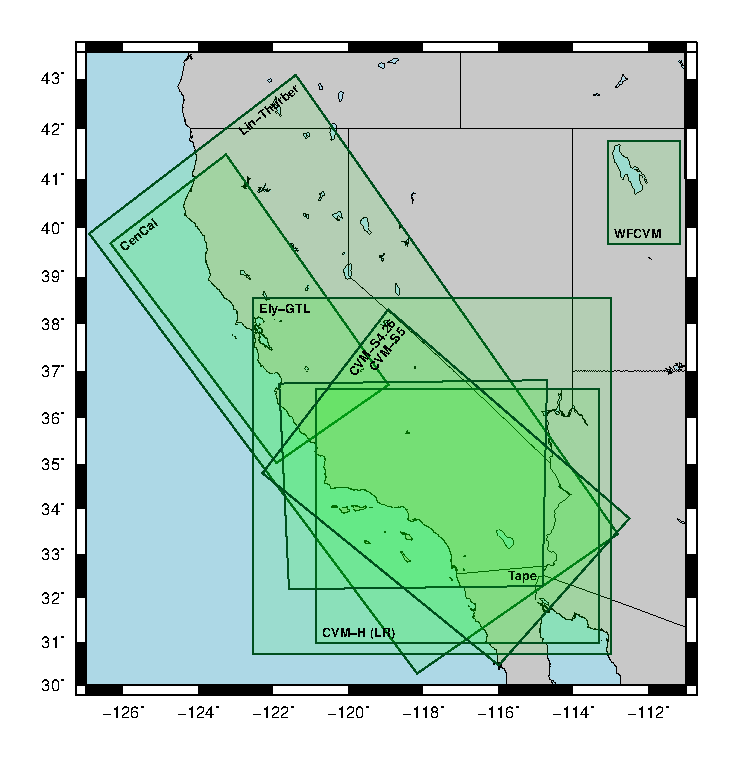
\includegraphics
		[width=0.7\textwidth]
		{figures/pdf/covered-areas}
	\caption{Surface horizontal projection of the areas covered by the various velocity models supported by the UCVM platform. See Table \ref{tab:cvms} for additional information and references.}
	\label{fig:cvms}
\end{figure*}


\section{Supported Velocity Models and Datasets}
\label{sec:cvms}

Existing geological velocity models vary considerably in terms of area of coverage, depth extent, composition, and resolution. The UCVM framework is flexible in its support for such variability and has been designed to integrate different velocity models, as well as to interact with their individual features seamlessly. UCVM has built-in support for a number of standard CVMs, which UCVM utilities identify through a series of corresponding string labels. Table \ref{tab:cvms} lists the models currently supported in the UCVM framework and provides additional details and references, along with their string labels. While all these models are supported by UCVM, only a fraction of them are included in the automated installation package. The remaining ones need to be installed manually before they can be accessed through the platform. Additional details are given in the documentation provided in Table \ref{tab:manuals} and in Section \ref{sec:easy.install}. In Table \ref{tab:cvms}, we indicate which of the models are included in the automated installation and which require manual installation. Figure \ref{fig:cvms} shows a map with the coverage areas of various CVMs.

UCVM is distributed with an easy installation method which runs a Python script (\texttt{ucvm\_setup.py}) that prompts the user about which of the automated models are to be installed (see Section \ref{sec:easy.install}). Before they are accessible through the UCVM framework, velocity models need to be enabled through a UCVM configuration file entry, and UCVM needs to be compiled. If the user wants to enable other velocity models at a later time, the framework needs to be compiled again in order to enable the desired additional models. Advanced users can also customize the installation to support other models, including user-defined velocity models, which can be added in the form of an \textit{etree} \citep{Tu_2003_Tech} database or as a \textit{patch} (rasterized) model. These advanced features and other options mentioned here are described in greater detail in the UCVM Advanced User guide (see Table \ref{tab:manuals}), and are controlled at run-time through a configuration file read by UCVM to identified the model(s) to be queried and the different alternative features.

In addition to standard velocity models, UCVM includes two geotechnical layer (GTL) models, also listed in Table \ref{tab:cvms}. These models are intended to supplement (i.e., modify or replace) the near-surface information in the original velocity models for a smoother transition from the softer near-surface soil deposits to the stiffer bedrock basement. The first of the two GTL models implements a \vsthirty-based interpolation from the free surface down to a given depth $z$, following \citet{Ely_2010_AGU}. The second GTL model is a generic one-dimensional (1D) model identical to the 1D crustal model. Two interpolation schemes can be used to smooth GTL material properties with the underlying crustal model material properties: a linear interpolation, or the interpolation relationship used by \citet{Ely_2010_AGU}. As in the case of the CVMs, the GTLs and the interpolation schemes are identified with string labels, \texttt{elygtl} and \texttt{1dgtl} for the \vsthirty-based and the 1D models, respectively. Similarly, the interpolation schemes are identified with the labels \texttt{ely} and \texttt{linear}. Note that the Ely GTL and interpolation models are used in the CVM-H model by default, with a reference depth of $z=350$~m. This option can be turned on or off for CVM-H by setting the model flag \texttt{USE\_GTL} \texttt{=} \texttt{true/false} in the configuration file.

To support the \vsthirty-based GTL model, UCVM has two built-in standard maps for California at 1 arcsec resolution (following USGS NED standards). These maps contain elevation data and \vsthirty{} data for the region indicated in Figure \ref{fig:cvms}. \vsthirty{} values are assigned following one of two possible options. Option one implements the procedure by \citet{Wills_2006_BSSA} and \citet{Wald_2007_BSSA}. Option two follows \citet{Yong_2012_BSSA}. These options are identified by the string labels \texttt{ucvm}, which is the default option, and \texttt{yong}. These maps are stored as etree databases, and their details are included in Table \ref{tab:cvms} and Figure \ref{fig:cvms}.

Since most models are bounded to a particular coverage area, UCVM provides alternative options to support background models. The CVM-S model, for instance, reverts to a 1D velocity model outside its defined region (see references provided in Table \ref{tab:cvms}). The UCVM-H model, on the other hand, is supported through UCVM with an optional background 1D velocity structure. This option allows queries at points outside and below the domain covered by the standard version of the model. While this option is inactive by default, it can be controlled manually by setting the model flag \texttt{USE\_1D\_BKG} \texttt{=} \texttt{true}. Other models can make use of this background structure by including the 1D model in the list of query models; that is, in the models sequence used to compose the meta-model. We refer to this process as tiling and explain its implementation in Section \ref{sec:querying}.

%\textcolor{green}{The USE\_1D\_BKG option applies only to CVM-H. If the user wants to use the default 1D background with UCVM, they need to provide it in the list of query models, following the main models that they are interested in.}

%various supplementary datasets and models that can be used in combination with the velocity models, or retrieved separately. The
%
%The standard 

%additional models are to be installed New velocity models can also be added to UCVM. 
%In addition to the standard CVMs, UCVM also provides access to two additional types of 
%
%various datasets that can be used to complement the functionality of the velocity models and provide supplementary information. Two types of additional datasets 
%
%
%(temp material)
%
%% However, in order to better accommodate high frequency ground motion simulations, it 
% 
%categorizes models into two general groups: crustal models, and geotechnical layers (GTLs). Crustal models provide subsurface seismic wave velocities associated with basin, crust, and mantle structures. These models may potentially extend to many tens of kilometers below the Earth's surface yet do so at coarse resolutions (TODO: cite CVM-H, CVM-S). Geotechical layers, in contrast, provide velocities for only the near-surface (typically a few hundred meters) at very high resolution (TODO: cite Ely Vs30 GTL). Ground motion simulations, in particular, rely on high-resolution near-surface velocities and therefore a GTL serves to supplement the coarser data provided by crustal models.
%
%TODO: Interpolation of GTL with Crustal

%\section{Material Models}
%\label{sec:velocity.models}
%
%We consider the same simulation domain used in \citet{Taborda_2013_BSSA}, wich consists of a volume of \vdomain{180}{135}{62}{km} that covers most of the Los Angeles metropolitan area, as show in Figs.~\ref{fig:earthquake}a and \ref{fig:source}a (left). We are interested in characterizing the material properties of the crustal structure and sedimentary basins within this volume, that is, the seismic velocities \vp{} and \vs{}, the material density $\rho$, and the quality factors \qp{} and \qs{} associated with the attenuation of $P$- and $S$-waves. Typical information about these properties comes in the form of velocity models, which provide information about \vp{}, \vs{} and $\rho$; and attenuation empirical rules that provide values of \qp{} and \qs{} as functions of \vp{} and \vs{}. In addition, some velocity models provide the option to include supplementary information about soft sedimentary deposits near the surface, also called geotechnical layers (GTL).
%
%Here, we use the community velocity models developed and supported by the Southern California Earthquake Center, CVM-S and CVM-H. In the case of CVM-H, we also consider an additional alternative that includes a GTL model. We refer to this latter model as CVM-H+GTL. It is worth mentioning that because of the history and original affiliation of the developers of the models, CVM-S is often referred to as the SCEC model, while CVM-H is often identified as the Harvard model. Hereafter, we will use the terms CVM-S, CVM-H and CVM-H+GTL when referring to the individual models; and at times speak of the Harvard models when indistinctly referring to CVM-H or CVM-H+GTL. The material's quality factors are based on an empirical rule. These models and the attenuation rule are described next.
%
%\subsection{CVM-S}
%
%We use CVM-S version 11.11.0. This version of CVM-S is equivalent to version 4.1 but includes additional improvements to the application programming interface (API). CVM-S is built upon the original work by \citet{Magistrale_1996_BSSA, Magistrale_2000_BSSA}. It integrates available information about the major southern California basins (Los Angeles Basin, Ventura Basin, San Gabriel Valley, San Fernando Valley, Chino Basin, San Bernardino Valley, and the Salton Trough). Outside and below the basins, CVM-S uses a 3D seismic tomography model \citep{Hauksson_2000_JGR} and an upper mantle model based on teleseismic inversions \citep{Kohler_2003_BSSA}. Inside the basins, it uses data from shallow and deep boreholes, oil wells, gravity observations, seismic refraction surveys, and other empirical rules based on the depths and ages estimated for a set of geological horizons.
%
%When queried at a particular longitude, latitude and depth, CVM-S provides the values of \vp{}, \vs{}, and $\rho$ for the specific query-point. In general, CVM-S operates by depth, in reference to the free surface, but does not provide information about the topography. We ignore the free-surface elevation and model the region in the simulation domain by flattening the topography \citep[see \textit{squashed topography} in][]{Aagaard_2008_BSSA1}. We access the information stored in CVM-S through the Unified Community Velocity Model (UCVM) software framework developed by SCEC \citep{Small_2011_AGU, Gill_2013_Proc}, and use additional utilities provided by UCVM to facilitate the simulation process (see \nameref{sec:approach}). 
%
%\subsection{CVM-H}
%
%We use CVM-H version 11.9.1. CVM-H is built upon the initial work by \citet{Suss_2003_JGR} and subsequent improvements by \citet{Suss_2005_SCEC} and \citet{Plesch_2007_SCEC, Plesch_2009_SCEC, Plesch_2011_SCEC}. It consists of a series of basin structures defined using seismic reflection profiles and tens of thousands of borehole measurements, and provides material properties comprised of various tomographic and teleseismic crust and upper mantle models. The basin structures in CVM-H are compatible with the geometry of major faults in southern California, as represented in the SCEC Community Fault Model \citep{Plesch_2007_SCEC}. The model also incorporated travel time tomographic information about the crust extending to a depth of 35 km, and upper mantle teleseismic and surface wave models extending to a depth of 300 km \citep{Prindle_2006_GJI}. Additional improvements to the model were included after a series of 3D adjoint tomographic inversions by \citet{Tape_2009_S}.
%
%CVM-H operates by elevation in reference to the sea level, but includes an internal elevation reference dataset to allow topographic flattening. We query the information in CVM-H by depth through the API provided with the UCVM, and rely on the internal algorithms of CVM-H and UCVM to do the conversion from depth to elevation to extract the values of \vp{}, \vs{} and $\rho$ at each longitude, latitude, and depth point of interest. In practice, CVM-H obtains these values from four volumes: a small high-resolution (HR) box which covers part, but not all of the Los Angeles metropolitan area, a low-resolution (LR) and crustal/mantle (CM) box which cover all of southern California and part of northern Mexico, Arizona and Nevada, and a background 1D model. By default, the current distribution of CVM-H also integrates the information of a GTL model. Here, however, we refer to CVM-H as the model with the GTL option \textit{inactive}. 
%
%\subsection{CVM-H+GTL}
%
%We use the term CVM-H+GTL to describe the CVM-H model with the GTL option \textit{active}. The CVM-H+GTL model is the same as CVM-H in reference to the HR, LR, CM and 1D models, but it incorporates supplementary information about the material properties in the near-surface geotechnical layers. The algorithm used to derive the values of \vp{}, \vs{} and $\rho$ in the GTL was introduced by \citet{Ely_2010_AGU}. It operates by replacing the information in the upper 350~m of the crustal velocity model with a model derived from \vsthirty{} maps. These maps provide a characteristic value of \vs{} for the upper 30~m near the surface. In particular, the GTL model in CVM-H combines information from the geology-based \vsthirty{} map developed by \citet{Wills_2006_BSSA} for California, and the slope-dependent (topography-based) estimation of \vsthirty{} by \citet{Wald_2007_BSSA} for points outside California.
%
%In summary, the GTL model works as follows. At the surface, the value of \vs{} is set to 0.5\vsthirty{} as derived from the \vsthirty{} maps, and the values of \vp{} and $\rho$ are determined using the empirical rules introduced by \citet{Brocher_2005_Tech}. Then, \vp{}, \vs{}, and $\rho$ are interpolated between the values at the surface and the values obtained from the HR/LR/CM/1D models in CVM-H at a transition depth, $z_{\mathrm{T}}=350$~m. The interpolation between the surface properties and the corresponding values at $z_{\mathrm{T}}$ combines a second order polynomial and a square-root function of depth. According to \citet{Ely_2010_AGU}, the generic interpolation curve was calibrated to produce a smooth and well-behaved transition in the profiles of selected sites in southern California.
%
%\begin{figure*}[!ht]
%	\centering
%	\includegraphics[width=\textwidth]{figures/pdf/figure-03}
%	\caption{Horizontal spatial distribution of the material's shear wave velocity in the region of interest at the free surface (top) and at 250~m in depth (bottom) for the CVM-S (left), CVM-H (center) and CVM-H+GTL (right) models. The rectangular box in the top-center frame indicates the boundaries of the high-resolution (HR) dataset used in CVM-H and CVM-H+GTL. The top-right frame includes labels for the location of the main basins, valleys and mountain ranges in the region of interest. The color version of this figure is available only in the electronic edition.}
%	\label{fig:hslices}
%\end{figure*}
%
%\begin{figure*}[!ht]
%	\centering
%	\includegraphics[width=\textwidth]{figures/pdf/figure-04}
%	\caption{Isosurfaces of different values of shear wave velocity for the three modeles considered here. From top to bottom, \vs{} = 500, 1500, and 2500 m/s; and from left to right the isosurfaces correspond to CVM-S, CVM-H and CVM-H+GTL. An additional frame at the top of the array indicates the location of the main basins, valleys and mountain ranges in the region of interest. The color version of this figure is available only in the electronic edition.}
%	\label{fig:isos}
%\end{figure*}
%
%\subsection{Models' Highlights}
%
%\refFig{fig:hslices} shows the horizontal distribution of \vs{} for the three models at the free-surface and at 250~m in depth. This figure highlights some of the differences in the models. At the free surface, for instance, it is clear that CVM-S and CVM-H have different boundaries for the underlying crustal structure and the basins within it. One major difference is in the deposits south and south-west from the Santa Ana Mountains and near the shore, which are absent in CVM-S. This differences also extend in depth. At 250~m, for instance, CVM-H has significantly more detail in the Los Angeles basin than CVM-S, whereas the Ventura Basin and Santa Clara River Valley seem to be better defined in CVM-S than in CVM-H. On the other hand, CVM-H and CVM-H+GTL are significantly different near the surface, where the GTL model prevails over CVM-H. These differences decrease with depth, as the interpolation function used for supplementing CVM-H with the GTL model approaches the transition depth, $z_{\mathrm{T}}=350$~m \citep{Ely_2010_AGU}. Beyond this depth, the two Harvard models become identical and differ equally from CVM-S. 
%
%Another point of interest is the contrast between the LR and HR model components in CVM-H and CVM-H+GTL. Our simulation domain is fully contained in the LR/CM/1D datasets of the Harvard models, but the HR box is smaller than our region of interest, as can be seen in \reffig{fig:hslices}. This figure shows that the transition between the HR and the LR models is not smoothly resolved, especially near the corner of the San Gabriel Valley and the boundary between the Los Angeles Basin and the San Fernando Valley.
%
%Further differences between the models are displayed in \reffig{fig:isos}, which shows isosurfaces for each model at values of \vs{} = 500, 1500 and 2500 m/s. The differences between CVM-H and CVM-H+GTL are rather subtle and concentrate on the \vseq{500} isosurface, where the changes introduced by the GTL model have the effect of deepening the horizon of these low velocity profiles. On the other hand, the differences between CVM-S and CVM-H(+GTL) are more significant. Some major differences are noteworthy. The Harvard models, for instance, define a deep sedimentary structure (with \vsleq{500}) offshore and to the west of the Santa Monica Mountains, which is inexistent in CVM-S. The shapes and depths of the Santa Clara River and Ventura basins are also different between CVM-S and CVM-H.  In CVM-H, these and the San Fernando and Simi valleys are all within a greater deep basin. In CVM-S, on the other hand, these structures are somewhat more independent of each other and there is no one major basin underneath.
%
%\subsection{Attenuation}
%
%Neither CVM-S nor CVM-H(+GTL) provide information about the material's internal friction properties. We rely on empirical rules available in the literature to define the material's quality factor, $Q$, based on values of \vp{} and/or \vs{}. There are different rules of the sort, which usually make a distinction between the attenuation of body and shear waves, thus providing individual \qp{} and \qs{} values, respectively. Some rules express \qs{} as a polynomial function of \vs{}, and \qp{} as a linear function of \qs{} or \vp{} \citep[e.g.,][]{Brocher_2005_Tech, Brocher_2008_BSSA, Olsen_2003_BSSA, Graves_2008_BSSA}. Here we use:
%%
%\begin{align}
%	\mathqs =\; 
%		& 10.5 - 16\mathvs + 153\mathvs^2 - 103\mathvs^3 
%		\nonumber \\
%		& + 34.7\mathvs^4 - 5.29\mathvs^5 + 0.31\mathvs^6
%	\label{eq:qs-rule}
%\end{align}
%%
%\noindent
%and
%%
%\begin{equation}
%	\mathqp = \frac{3}{4}\left( \mathvp / \mathvs \right)^2 \mathqs
%	\hspace{.25em}.
%	\label{eq:qp-rule}
%\end{equation} 
%
%The expression for \qs{} given by equation \refeqn{eq:qs-rule} was designed as a smooth alternative to other $Q$-rules available in the literature \citep{Taborda_2013_BSSA}. Equation \refeqn{eq:qp-rule}, on the other hand, is derived from the special case in which one considers no attenuation due to dilatational deformation, i.e., $Q_\kappa \rightarrow \infty$ \citep[e.g.,][]{Stein_2003_Book, Shearer_2009_Book}. Although there is an ongoing discussion about the extent of validity of these and other similar rules, we adopt the aforementioned expressions for consistency with our previous simulation of the Chino Hills earthquake. 
%
%






%\textit{
%\color{blue}
%This section will present how CVMs work and the various CVMs available to the community today. It will basically explain that CVMs provide the triplets of Vs, Vp and density, and, as an example, we can expand on a description of CVM-S and CVM-H, including their variations CVM-SI and CVM-H+GTL.
%}









\subsection{Utilities}

\subsubsection{Querying}

\subsubsection{Gridding and Meshing}

\subsubsection{UCVM and the Etree Library}

\subsubsection{New DEMs and Vs30 Maps}

\subsection{Parallel Utilities}

\subsection{Application Programming Interface}


\section{Computational Performance}
\label{sec:conclusions}

\textit{
\color{blue}
It would be desirable to do some experiments in terms of performance, especially for the parallel applications utilities in UCVM. With some examples of how long the same thing would take if doing it differently. We will need to discuss this.
}

\section{Recent Case Applications}
\label{sec:conclusions}

\textit{
\color{blue}
This section will be dedicated to show case applications. Some ideas for potential subsections follow.
}

\subsection{Visualization and Model Comparisons}

\subsection{Chino Hills Simulation Series}

\subsection{CyberShake}

\section{Summary and Conclusions}
\label{sec:conclusions}

\textit{
\color{blue}
A couple of paragraphs with a summary of what is shown in the paper and a few key conclusions about the impact that we expect UCVM has already have and will have on earthquake research.
}

